\documentclass[11pt, a4paper]{arbeitsblatt}

\ladeModule{theme,qrcodes,muster}
\ladeFach[]{mathematik}

\aboptionen{
	name		= {J. Neugebauer},
	kuerzel 	= {Ngb},
	titel 		= {Winkelsumme im Dreieck},
	reihe 		= {Kongruenz},
	fach 		= {Mathematik},
	kurs 		= {Jg.7},
	nummer 		= {V.2},
	lizenz 		= {cc-by-nc-sa-4},
	version 	= {2021-06-06},
}


\begin{document}
\ReiheTitel

\begin{aufgabe}[icon=\iconTablet\,\iconPartner]
	\label{aufg:vermutung-aufstellen}
	Konstruiert in \programm{Sketchometry} ein Dreieck und markiert die drei
	\emph{Innenwinkel}. Messt die Winkel sowie die Summe der Winkel und platziert
	die Winkelmaße auf der Zeichenebene.

	Verändert die Form des Dreiecks durch Ziehen an einem der Eckpunkte und
	beobachtet die Winkelmaße.

	\hinweis{Ihr könnt die Summe von mehreren Winkeln messen, indem ihr die Winkel
	nacheinander antippt.}

	Notiert eine Vermutung zur Summe der Innenwinkel in einem Dreieck im Heft.
\end{aufgabe}

\begin{wrapfix}
\begin{wrapfigure}[5]{r}[5mm]{0pt}
	\qrcode{https://qr-lernhilfen.de/mobileUrl?url=508f77f12aaf9c38}
	% \caption*{\scriptsize Tipp}
\end{wrapfigure}
\begin{aufgabe}[icon=\iconTablet\,\iconPartner]
	\label{aufg:konstruktion}
	Ergänzt eure Konstruktion wie in \prettyref{abb:konstruktion} gezeigt.

	\begin{itemize}
		\item Zeichnet Geraden durch die Eckpunkte des Dreiecks.
		\item Zeichnet eine Parallele zu jeder Geraden, die durch den jeweils gegenüberliegenden
		Eckpunkt des Dreiecks verläuft.
	\end{itemize}

\begin{figure}[h]\centering
	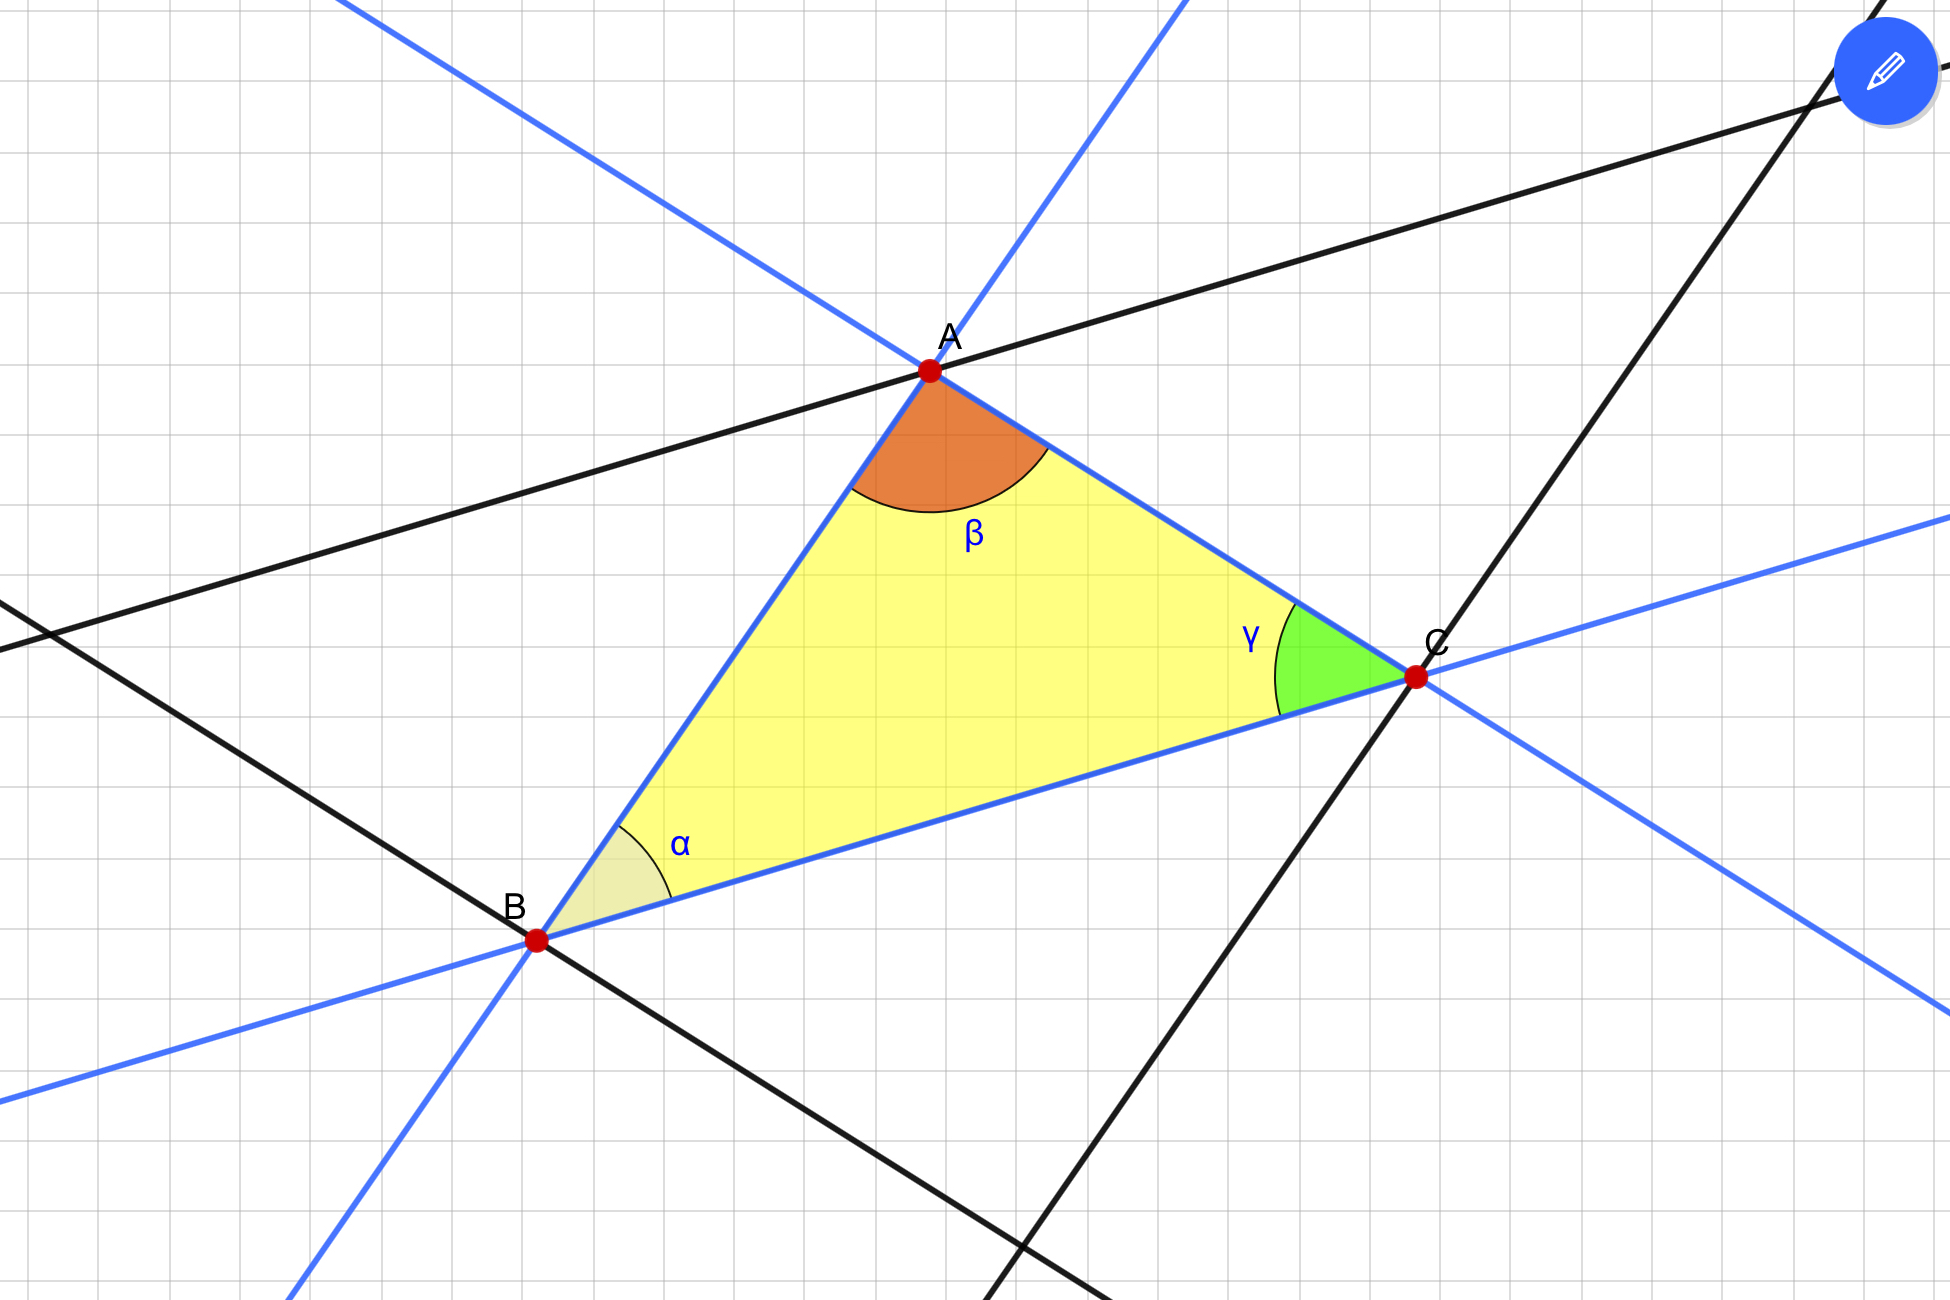
\includegraphics[width=.4\linewidth]{Jg.7-AB.02-Abb_Konstruktion.jpeg}
	\caption{Konstruktion in \programm{Sketchometry}}\label{abb:konstruktion}
\end{figure}
\end{aufgabe}
\end{wrapfix}

\begin{wrapfix}
\begin{wrapfigure}[3]{r}[5mm]{0pt}
	\qrcode{https://qr-lernhilfen.de/mobileUrl?url=0af735e5cf203a92}
	% \caption*{\scriptsize Tipp}
\end{wrapfigure}
\begin{aufgabe}[icon=\iconTablet\,\iconPartner]
	\label{aufg:vermutung-beweisen}
	Findet einen Weg, um anhand der Konstruktion zu zeigen, dass die Vermutung
	aus \prettyref{aufg:vermutung-aufstellen} korrekt ist. \\
	Nutzt dazu euer Wissen über Winkelbeziehungen.
\end{aufgabe}
\end{wrapfix}

\begin{aufgabe}[icon=\iconStift\,\iconPartner]
	\label{aufg:beweis-notieren}
	Haltet eure Begründung mit einer Skizze im Heft fest. Übernehmt nur Elemente,
	die für eure Begründung wichtig sind.
\end{aufgabe}

\begin{wrapfix}
\begin{wrapfigure}[5]{r}[5mm]{0pt}
	\qrcode{https://qr-lernhilfen.de/mobileUrl?url=02fc217731ac8402}
\end{wrapfigure}
\begin{aufgabe*}[icon=\iconTablet\,\iconPartner]
	\label{aufg:n-ecke}
	Stellt Vermutungen für die Winkelsumme von Vierecken auf
	und prüft sie mit \programm{Sketchometry}. Könnt ihr eure Vermutungen auch
	Begründunden?

	Welche Winkelsumme hat ein allgemeines $n$-Eck?

	\tipp{Überlegt, wie man ein $n$-Eck in Dreiecke zerlegen kann.}
\end{aufgabe*}
\end{wrapfix}

\end{document}
